
\section{GSM}

\subsection{Fixed-line phone networks}
Fixed-line phone networks were originally circuit-switched
\begin{center}
    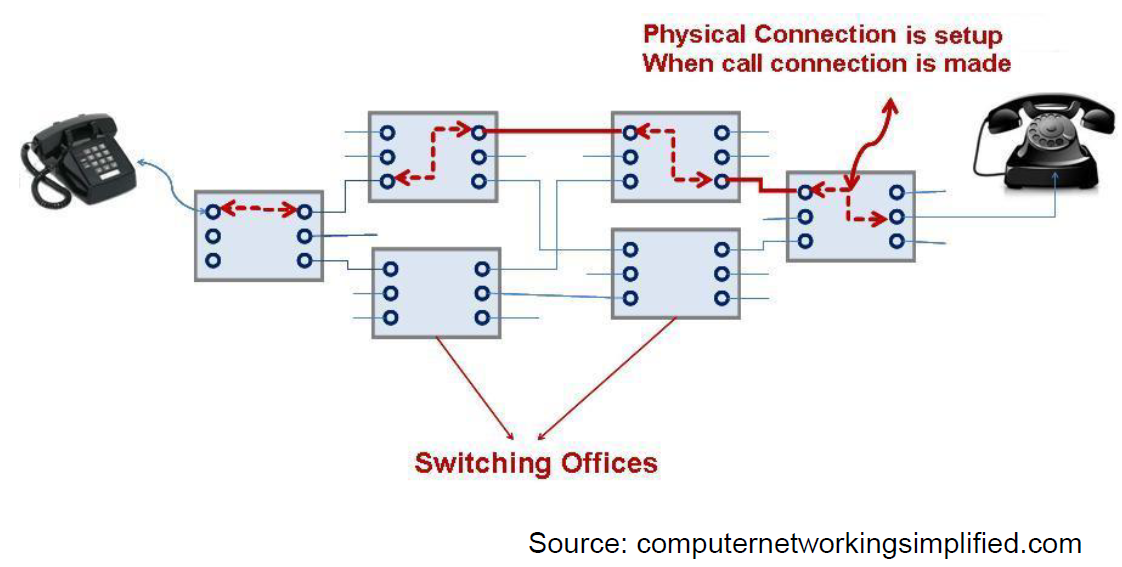
\includegraphics[width=0.5\linewidth]{img/fixed-line.png}
\end{center}
Connections were set up or teared through signaling protocol which information
exchange establish a connection. 

\subsubsection{Signaling protocols}
Two kinds of signaling protocols:
\begin{itemize}
\item \textbf{In-Band:} Signaling uses the same channel as the voice data
        \begin{enumerate}
            \item Human operator
            \item Pulse dialing
            \item Tone dialing
        \end{enumerate}

        \begin{itemize}
                \proitem{} Easy to implement 
                \consitem{} Fraud: end user can hack the signaling by
                creating the right pulse or tone sequence
        \end{itemize}

        SS5 (Signaling System No. 5) : set of protocols for in-band
        signaling

\item \textbf{Out-Band:} Separate digital channel and voice/data

        SS6 which used out-band was replaced by the more flexible and
        powerful SS7 which used out-band.
\end{itemize}

\subsubsection{SS7}
SS7 is a packet-switched protocol:
\begin{itemize}
    \item Message for call setup and tear down
    \item Also used for other kind of management information (billing,
        SMS,...)
\end{itemize}

\paragraph{Protocol stack}: Protocol stack similar to IP:
\begin{itemize}
    \item MTP-1 (Message Transfer Part 1): Physical layer
    \item MTP-2: data link layer, defines packets
    \item MTP-3: packet routing, packet have source and destination
        address called \textcolor{red}{point codes}
\end{itemize}
\begin{center}
    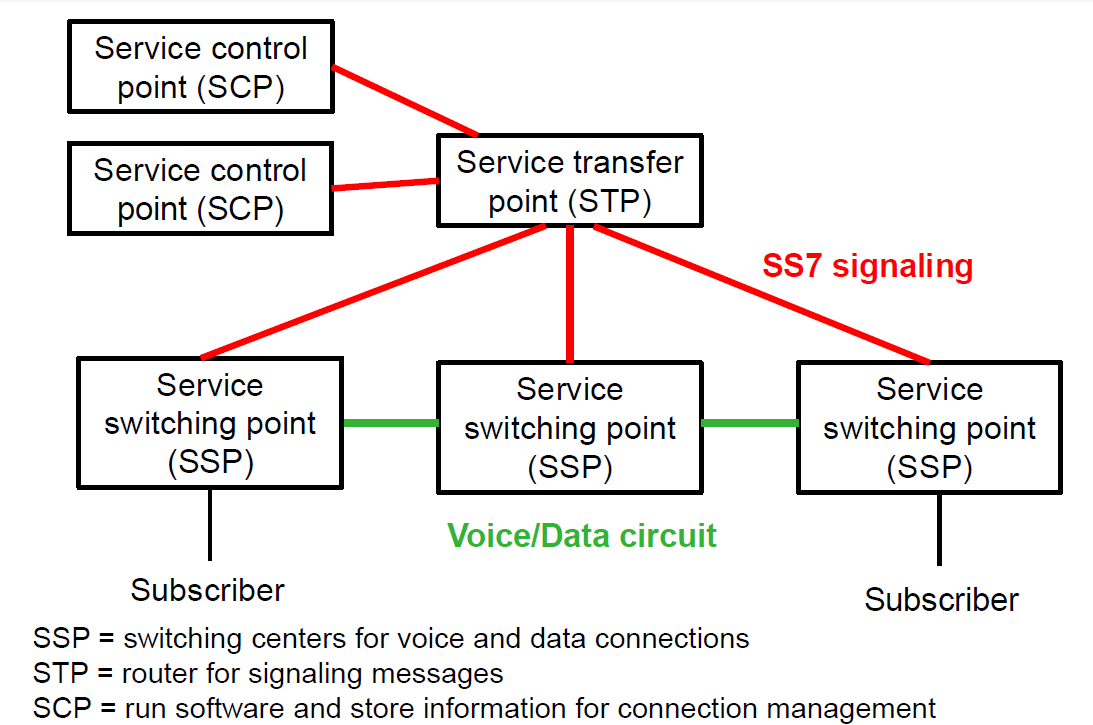
\includegraphics[width=0.5\linewidth]{img/ss7.png}
\end{center}

\begin{itemize}
    \item MTP-1 to MTP-3 only define basic signaling functionality
    \item There are other protocols that run on higher layers, for example protocols for core 
        network management, mobile call management, \ldots
    \item Nowadays SS7 runs over IP.
        \begin{itemize}
            \item MTP-1 replaced by Ethernet
            \item MTP-2 and MTP-3 replaced by IP/SCTP/...
        \end{itemize}
\end{itemize}


\subsection{GSM Component}
Global System for Mobile Communication, uses \textbf{SDMA},
\textbf{TDMA} and \textbf{FDMA}.
\begin{figure}[ht!]
    \centering
    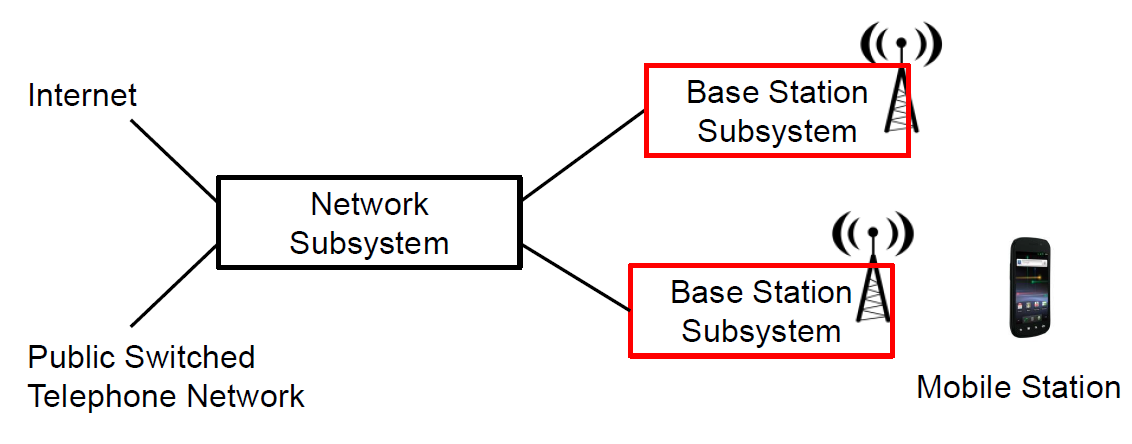
\includegraphics[width=0.6\linewidth]{img/gsm.png}
\end{figure}

\subsubsection{Base Station Subsystem}
The base station subsystem contains all necessary components for the radio
communication.

\begin{center}
    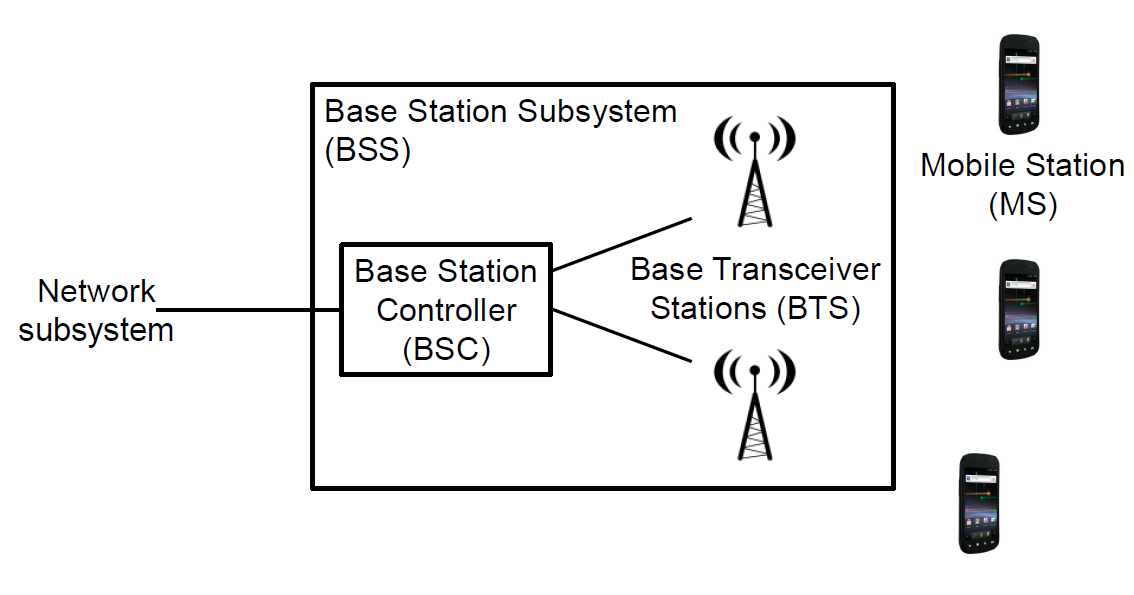
\includegraphics[width=0.6\linewidth]{img/bss.png}
\end{center}

\begin{description}
    \item[Base Station Controller:] Control item such as handover and allocate
        channel for a call
    \item[Base Transceiver Station:] Radio Transmitter that can cover an area (cell) with
                radius of up to 35 km but can only serve limited number of users. 
        \begin{itemize} 
            \item Each BTS can use only a limited number of frequencies 
                because of interferences with neighbor cells
            \item To increase capacity, the coverage area of a BTS is usually
                split into two or three sectors
                \begin{center}
                    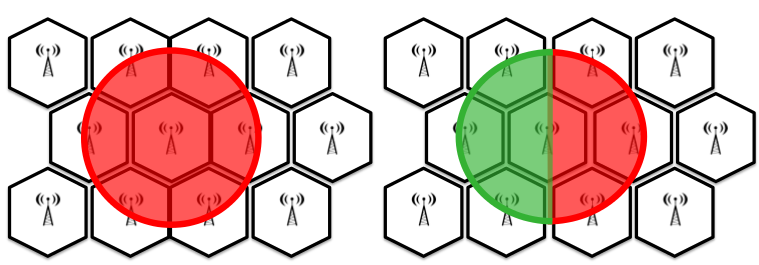
\includegraphics[width=0.4\linewidth]{img/cellular.png}
                \end{center}
        \end{itemize}


\end{description}

\paragraph{Characteristics}

\begin{itemize}
    \item \textbf{Frequency Band}
        \begin{itemize}
            \item \textit{GSM-900}:
                \begin{itemize}
                    \item 124 downlink carrier frequencies from 935.2 MHz to 960MHz( BS to MS)
                    \item 124 uplink carrier frequencies form 980.2 MHz to 915 MHz (MS to BS)
                    \item Each channel 200kHz bandwidth
                    \item 2 Watt transmission power in handset
                \end{itemize}

            \item \textit{GSM-1800}: 374 channels 1710-1880Mhz
        \end{itemize}

        $\Rightarrow$ For cost reasons, a GSM mobile station operates on
        only one frequency at a time, it can either receive or transmit
        at a time.

    \item \textbf{Timeslots}: Each carrier frequency is divided into 8
        repeating timeslot (\textcolor{red}{burst}) of 0.577ms
        $\Rightarrow$ \textbf{TDMA}

        \begin{itemize}
            \item The 8 timeslots of a carrier frequency are called
                \textcolor{red}{physical channel}, channel are
                identified by its frequency and timeslot number

            \item Number of physical channels determines how many simultaneous active MS the 
                base station can handle
        \end{itemize}
        During a timeslot, burst are sent. 

        \paragraph{Burst structure} 
        There exists different type of burst (synchronization,
        voice/datan...). For a normal burst used for voice and data 
        the structure is:
        \begin{center}
            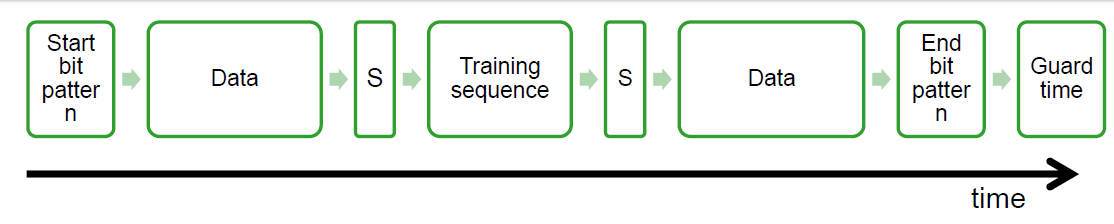
\includegraphics[width=0.8\linewidth]{img/burst-structure.png}
        \end{center}

        \begin{description}
            \item[Start bit pattern] Gives time for the transmitter to ramp up its power
            \item[Data] 2 fields of 57 bits carrying information
            \item [S bits] One for each data field indicating that the data fields contain
                urgent signaling information instead of normal data
            \item [Training data] contains a fixed bit pattern, used by the receiver to 
                optimize its filter parameters in order to compensate for interferences
            \item [End bit pattern] Gives time for the transmitter to ramp down its power
            \item[Guard time] Prevent overlap between burst
        \end{description}

        \paragraph{Timing}
        TDMA requires \textbf{exact timing} but signal propagation time depends on distance
        between phone and base station. 
        \begin{itemize}
            \item Guard times at the end of the Normal Burst help but they are very
                short in GSM
            \item[$\Rightarrow$]Base Station measures the delay and
                sends signaling information to phone to adjust its
                timing
        \end{itemize}
\end{itemize}

\subsubsection{Logical Channels}
A logical channel (mapped to the physical channels) is channel dedicated to a specific type of 
information. Ex:
\begin{description}
    \item[TCH(Traffic Channel):] carries the voice and user data from/to a 
        mobile station
    \item[BCCCH(Broadcast Common Controm Channel):]used by the base station to 
        broadcast status information to all idle mobile stations
    \item[PCH(Paging Channel):] informs mobile stations about incoming calls or SMS
\end{description}

\paragraph{Mapping}

\begin{itemize}
    \item Compared to the traffic channel most logical signaling channel only carry few 
        information and therefore can be time-multiplexed on the same physical 
        channel:
        \begin{itemize}
            \item Typically, timeslots 0 and 1 of the first frequency of a base station are 
                used for signaling channels
            \item The other timeslots and frequencies are used for the traffic channel
            \item The base station manages the mapping
        \end{itemize}

    \item We than have \textbf{common} channels that can be used by all MS
        and \textbf{dedicated} channels assigned to specific MS.
\end{itemize}

%TODO: Example slide 22 for GSM

\paragraph{Example: Traffic Channel}
A dedicated channel used for voice or user data:
\begin{itemize}
    \item Full rate: 13 kbit/s
    \item Half rate: 6.5 kbit/s, two MS share a timeslot
\end{itemize}

When allocating the TCH for a MS, the BSC chooses timeslots in the down-link
frequency and the up-link frequency that are at least 3 timeslot periods
apart.

\begin{itemize}
    \item MS has enough time to switch from the down-link frequency to the
        up-link frequency
    \item MS needs only one transceiver
\end{itemize}

\subsubsection{Network Subsystem}
\begin{figure}[ht!]
    \centering
    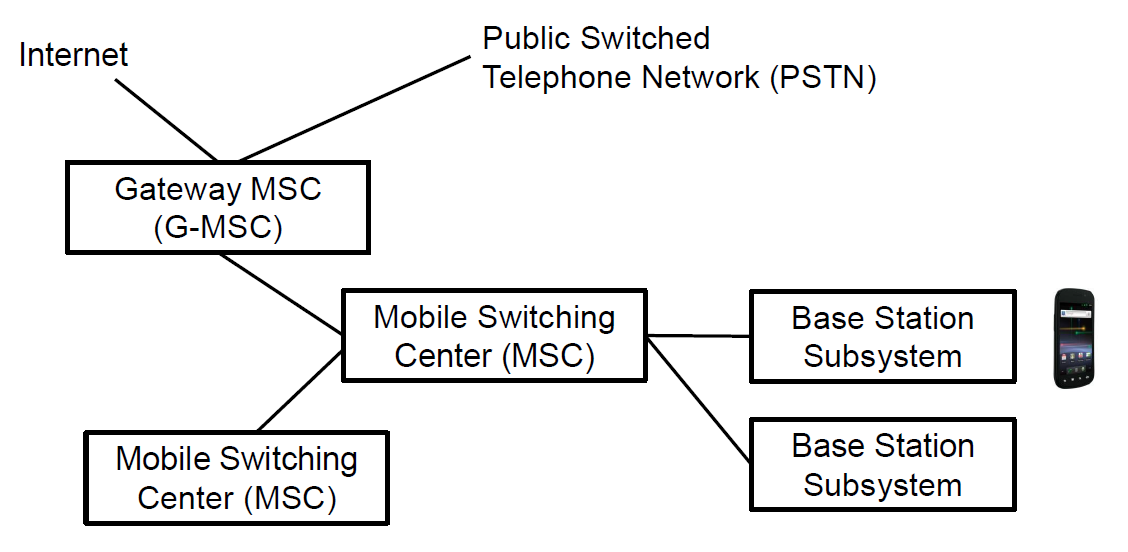
\includegraphics[width=0.7\linewidth]{img/nss.png}
    \caption{Signaling with SS7 protocols running on top of MTP-3}
\end{figure}

\begin{description}
    \item[Mobile Switching Center:] MSCs are responsible for switching phone
        calls between mobile stations or with fixed-line phones. Responsible for
        one or several BSS
    \item [Gateway-MSC:] The same as MSC but with a gateway to Public Switched
        Telephone Network (PSTN).
\end{description}

Since MS can roam freely between cells and even between operators, the MSC
must keep track of the location of the MS, otherwise, calls to the MS can not be
routed to the right BSS.

\paragraph{Informations stored}
An MSC has access to several detabases that store information about subscribers:
\begin{itemize}

    \item \textbf{Equipment Identity Register (EIR):} List of blocked, faulty,
        to-be-monitored device

    \item \textbf{Home Location Register (HLR):} it is the subscriber
        central database of a GSM network, it contains a record for each
        subscriber (Each subscriber has a home area that served by
        exactly one HLR). A record contains for each SIM card:

        \begin{itemize}
            \item International Mobile Subscriber Identity (IMSI) = Unique ID
            \item One or more Mobile Subscriber International ISDN Numbers = Phone numbers
            \item Profile data (name, roaming limits etc.)
            \item Temporary data: current \textcolor{red}{VLR,MSC} 
        \end{itemize}

        $\Rightarrow$ \textbf{master table of the GSM operator,
        containing a record for each subscriber}

    \item \textbf{Visitor Location Register (VLR)}: Local database to
        reduce signaling between MSC and HLR. 

        \begin{itemize}
            \item It contains information from HLR when MS enters the
                VLR's service area (each BS served by exactly one VLR):
                \begin{itemize}
                    \item Subscriber's ID number and phone number
                    \item Service profile
                    \item HLR address
                    \item Roamin number: temporary phone number that can be used to find MS 
                        (MSC number)
                    \item \ldots
                \end{itemize}

            \item Typically implemented in the MSC
            \item Location area identity to further reduce signaling
                with HLR
        \end{itemize}

    \item Localization: Service areas are divided into smaller location
        areas (LA).

        $\Rightarrow$ Small mobility of subscriber does not cause remote HLR update

        \begin{center}
            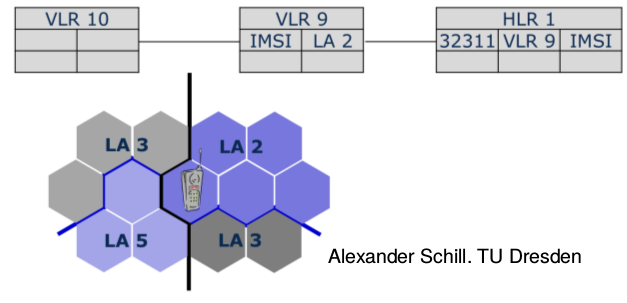
\includegraphics[width=0.8\linewidth]{img/localization.png}
        \end{center}

\end{itemize}

\paragraph{IMSI and MSIDN}
IMSI is the key identifying a SIM card, it stored in the HLR and on the SIM card
but the MSIDN (phone numbers) are not stored on SIM card.

\begin{tabular}{cm{10cm}}
    When MS is switched on:&
    \begin{enumerate}
        \item MS sends IMSI to MSC
        \item MSC analyses the country code and network code
        \item MSC sends request to HLR to retrieve the record
    \end{enumerate}
\end{tabular}

$\Rightarrow$ Advantages of separating IMSI and MSISDN: MSISDN can be
changed afterwards

\subsubsection{Handover}

Because MS can move freely, so MS can move from one cell to
another. BSC can decide to de a handover based on signal quality:

\begin{itemize}
	\item BTS constantly measures signal quality and reports to BSC
	\item MS also reports quality of signals it receives from other cells
\end{itemize}

\paragraph{Scenarios} 3 different scenarios:
\begin{itemize}
	\item Intra-BSC handover: old and new cell connected to same BSC
	\begin{enumerate}
		\item BSC activates a TCH in new cell
		\item BSC informs LS via old cell to handover to new TCH
		\item Once MS and BTS have confirmed handover, BSC redirects
		voice data to new cell and deallocates old TCH
	\end{enumerate}

	\item Inter-BSC handover: old and new cell connected different BSCs,
	but same MSC
	\begin{enumerate}
		\item BSC of old cell asks MSC to initiate handover
		\item MSC asks BSC of new cell to prepare a TCH
		\item MSC notifies MS to handover
		\item Once MS and BSC have confirmed handover, MSC redirects voice
		data and tells old BSC to close old TCH
	\end{enumerate}

	\item Inter-MSC handover
	\begin{enumerate}
		\item Old MSC sends handover request to new MSC
		\item New MSC contacts new BSC to establish TCH
		\item MSC notifies MS to handover
	\end{enumerate}
	The first MSC still stays responsible for the call, the call is routed from
	the G-MSC through the anchor MSC to the new MSC
\end{itemize}

\subsubsection{Security}
GSM security consist of Authentication and encryption:

\begin{itemize}
	\item \textbf{Authentication:} MS is authenticated

        Symmetric Key Ki(max. 128 bits) for IMSI stored in SIM
        card and in Authentication Center
        \begin{enumerate}
            \item Authentication Center generates:
                \begin{itemize}
                    \item a 128 bit random number RAND
                    \item a 32-bit signed responses SRES = A3(Ki,RAND)
                \end{itemize}
            \item MSC sends RAND to MS
            \item SIM card also computes SRES
            \item Response sent back to MSC
            \item MSC compares responses
        \end{enumerate}
        The A3 algorithm is not standardized. 
        \begin{itemize}
            \item New RAND and SRES generated for each authentication
            \item For speed-up, several RAND/SRES computed  in advance and
                buffered in MSC and VLR
        \end{itemize}

    \item \textbf{Encryption:} Communication between MS and BTS is encrypted

        Data exchanges between MS and BTS are encrypted,
        \begin{itemize}
            \item Creation of a 64-bit session key Kc = A8(Ki,RAND) by the 
                Authentication center
            \item MSC sends RAND to MS, so MS can also compute Kc
            \item Session key can be changed, at reqular intervals
        \end{itemize}
        MSC and MS use Kc and A5 algorithm to encrypt/decrypt data.
        A5 is a set of algorithms A5/1, A5/2...
        \begin{itemize}
            \item Input:
                \begin{tabular}{m{10cm}}
                    Kc\\
                    Current frame number N: different for every burst
                \end{tabular}
            \item Output:
                \begin{tabular}{m{10cm}}
                    114-bit sequence C=A5/x(Kc,N)
                \end{tabular}

            \item Encryption:
                \begin{tabular}{m{10cm}}
                    Encrypted burst = Original burst data XOR C
                \end{tabular}
        \end{itemize}
\end{itemize}

The keys of IMSI are stored in Authentication Center and in SIM card
and algorithm are implemented in the GSM network and on the SIM
card.

\paragraph{Strength and Weaknesses}
\begin{itemize}
        \proitem{} Keys and key generation inside SIM card, not by phone software
		\consitem{} A3/A5/A8 algorithm were secret and not publicly discussed
		\consitem{} 128 bit key length: Too short for modern computers
		\consitem{} Communication between BTS and BSC not encrypted
		\consitem{} MS is authenticated to network but not vice versa
		\consitem{} Network operator knows all keys
		\consitem{} No end-to-end authentication \& encryption
\end{itemize}

